%-------------------------------------------------------------------------------
\section{Analysis strategy}
\label{sec:strategy_Htautau}
%-------------------------------------------------------------------------------

The analysis strategy adopted in the $\Htautau$ search is similar to the one used in Ref.~\cite{fcnc36,Chen:2015nta} but extended to more search channels.

\subsection{Event categorisation and kinematic reconstruction}
\label{sec:htautau_reco_cat}

The $tt(qH)$ and $tH$ signal being probed is characterised by the presence of $\tau$-leptons from the decay of 
the Higgs boson and the remaining SM $t\to Wb$ decay. There is an additional $q$-jet from the FCNC $t\to qH$ decay in the top pair production. 
%at least  four (three) jets in the decay (production) mode, only one of which originates from a $b$-quark.
If the $W$ boson or one of the $\tau$-leptons decays leptonically, an isolated electron or muon with significant $\met$ is also expected.
In a significant fraction of the events, the smaller jet from the hadronic $W$ boson decay fails the minimum $\pt$ requirement of $25~\gev$,
resulting in some signal events mixed with production mode having only three reconstructed jets.
In order to optimise the sensitivity of the search, the selected events are categorised into seven SRs based on the number of light leptons,
$\had$ candidates, and on the number of light flavored jets:
$t_l\hadhad$, $t_l\had$-1j, $t_l\had$-2j, $t_h\lephad$-2j, $t_h\lephad$-3j, $t_h\hadhad$-2j, and $t_h\hadhad$-3j, as shown in Table~\ref{tab:srcr}. 

\begin{table}
\centering
\caption{Overview of the signal regions and the control regions used for fake tau scale factor derivation in leptonic channels.}
\label{tab:srcr}
\begin{tabular}[h]{c|c|c|c|c|c|c}
\hline \hline
\multicolumn{2}{c|}{Regions} & b-jet & light flavor jets        & lepton & hadronic taus & charge\\ \hline
\multirow{7}{*}{SR}&$t_l\thadhad$     & 1     & any                                & 1      & 2             & $\thadhad$ OS\\ \cline{2-7}
&$t_l\tauhad$-1j  & 1     & 1                                   & 1      & 1                     & $t_l\tauhad$ SS\\ \cline{2-7}
&$t_l\tauhad$-2j  & 1     & 2                                        & 1      & 1                     & $t_l\tauhad$ SS\\ \cline{2-7}
&$t_h\tlhad$-2j   & 1     & 2                           & 1      & 1             & $\tlhad$ OS\\ \cline{2-7}
&$t_h\tlhad$-3j   & 1     & $\ge3$                      & 1      & 1             & $\tlhad$ OS\\ \cline{2-7}
&$t_h\thadhad$-2j & 1     & 2                            & 0      & 2             & $\thadhad$ OS\\ \cline{2-7}
&$t_h\thadhad$-3j & 1     & $\ge3$                       & 0      & 2             & $\thadhad$ OS\\ \hline
\multirow{6}{*}{CRtt}&$t_lt_l1b\tauhad$ & 1     & any                           & 2      & 1                     & $t_lt_l$ OS\\ \cline{2-7}
&$t_lt_l2b\tauhad$      & 2     & any                           & 2      & 1                     & $t_lt_l$ OS\\ \cline{2-7}
&$t_lt_h2b\tauhad$-2jSS & 2     & 2                             & 1      & 1             & $t_l\tauhad$ SS\\ \cline{2-7}
&$t_lt_h2b\tauhad$-2jOS & 2     & 2                             & 1      & 1             & $t_l\tauhad$ OS\\ \cline{2-7}
&$t_lt_h2b\tauhad$-3jSS & 2     & $\ge3$                        & 1      & 1             & $t_l\tauhad$ SS\\ \cline{2-7}
&$t_lt_h2b\tauhad$-3jOS & 2     & $\ge3$                & 1      & 1             & $t_l\tauhad$ OS\\ \hline
\end{tabular}
\end{table}

%This event categorisation is primarily motivated by the different quality of the event kinematic reconstruction, depending on the amount 
%of $\met$ in the event (larger in $\lephad$ events compared with $\hadhad$ events), and whether a jet from the hadronic top-quark decay 
%is missing or not (events with exactly three jets or at least four jets).
This event categorisation is primarily motivated by optimizing the sensitivity in each signal region that targets both leptonic and hadronic top-quark
decays as well as the Higgs decays into $\lephad$ or $\hadhad$ final state.   
The event kinematic reconstruction is further applied in the $t_h\hadhad$ and $t_h\lephad$ channels to suppress the background by constraining the
di-tau mass and the missing transverse energy in the event~\cite{Chen:2015nta}. 
%based on the strategy used in Ref.~\cite{Chen:2015nta}, and is summarised below.

For the $t_ht(qH)$ events, the jet from $t\to qH$, denoted as the FCNC jet, should be a hard narrow jet considering it's from the
decay chain $t\to qH\to q\tau\tau$, with taus reconstructed as $\lephad$ or $\hadhad$.
There should be at least four jets among which with the closest angular distance to the visible decay of the di-taus
is considered as $q$-jet since the FCNC top decay products are likely boosted closer together than other jets. 
If there are more than 2 jets beside $q$-jet and $b$-jet, the jets from $W$ boson decay are chosen from the combination
with the invariant mass closest to W resonance. There is the chance that one of the jets fails the $\pt$ requirement and not reconstructed. This kind of events will fall
into $t_hH$.
%while the FCNC top resonance is
%still reconstructable that the missing jet is likely from the decay of $W$ boson.
%given the big chance that the jet which is missing is from $W$ decay.

In the $t_hH$ events, there are 3 jets coming from top hadronic decay including the b-jet. So a Higgs resonance formed by the taus and a top resonance formed by
the jets are expected.

Finally, the four-momenta of the invisible decay products from the decay of di-taus 
are estimated using a kinematics fit. The fit is done by minimising a $\chi^2$ function based on the Gaussian constraints on the Higgs boson mass and the
measured $\met$ within their expected resolutions. The resolution on the Higgs boson mass is taken to be $20~\gev$, respectively, while the resolution on the measured $\met$ is parameterised as a linear function of 
$\sqrt{\sum E_T}$, where $\sum E_T$ is the scalar sum of the $\pt$ of all physics objects contributing to the $\met$ reconstruction~\cite{Aaboud:2018tkc}.
After the $\chi^2$ minimisation, the Higgs boson four-momentum, and hence its invariant mass, as well as the 
four-momentum of the parent top quarks, are determined with better resolution in the signal events. 

For the  $t_lt(qH)$ and $t_lH$ events where the $W$ boson from $t\to W b$ decays leptonically, there is a neutrino with large momentum and the flying direction is unknown. The kinematics fit is no longer feasible in the $t_l\hadhad$ and $t_l\had$ channels. The kinematic variables are calculated using the visible
objects only.

With the event topology reconstructed, a number of variables are defined for signal and background separation used in the multivariate analysis discussed below.

%In the  $t_lt(qH)$ and $t_lH$ signal, the additional $q$ jet in the decay mode can still be found, but since the $W$ boson decays leptonically, there is a neutrino with large momentum and the flying direction is unknown. The kinematics fit is no longer feasible in the $t_l\hadhad$ channel. The variables calculated from the visible objects are directly used in the multivariate analysis. However, the kinematics fit is still performed for the $t_l\had$ channels where the lepton and $\had$ are treated as di-tau candidate.

\subsection{Multivariate discriminant}

%%%%%%%%%%%%%%%
\begin{table*}[t!]
\caption{\small{$\Htautau$ search: Discriminating variables used in the training of the BDT for hadronic channel. 
    The descriptions of each variable are provided in the following text.}}
\label{tab:importance_xTFW}
\centering
\begin{tabular}{ccc} \toprule\toprule
  & $t_h\thadhad$-2j & $t_h\thadhad$-3j\\\midrule
$m_{\text{W}}$                               & $7.62$ / $6.54$ & $7.00$ / $8.00$\\
$m_{\text{t},\text{SM}}$                            & $10.61$ / $10.55$ & $9.66$ / $9.64$\\
$p_{\text{T},\tau }$                         & $5.70$ / $6.96$ & $5.86$ / $5.13$\\
$\met$                        & $7.07$ / $5.76$ & $4.34$ / $5.77$\\
$m_{\tau\tau,\text{vis}}$                  & $10.72$ / $10.95$ & $11.26$ / $10.92$\\
$m_{\tau ,\tau }$                     & $14.36$ / $14.63$ & $14.77$ / $13.77$\\
$m_{\text{t},\text{FCNC}}$                          & $5.81$ / $7.01$ & $7.49$ / $8.24$\\
$\Delta R(\tau,\tau)$               & $10.27$ / $9.58$ & $10.00$ / $9.12$\\
$\Delta\phi(\tau\tau,\met)$ & $2.69$ / $5.71$ & $4.51$ / $5.03$\\
$\met \text{centrality}$             & $3.89$ / $4.68$ & $5.87$ / $5.51$\\
$E_{\text{vis}~\tau ,1}/E_{\tau ,1}$         & $6.56$ / $5.50$ & $6.32$ / $4.74$\\
$E_{\text{vis}~\tau ,2}/E_{\tau ,2}$         & $6.45$ / $5.21$ & $4.72$ / $7.37$\\
$\Delta R(\tau,\text{light-jet})$       & $8.26$ / $6.93$ & $8.20$ / $6.75$\\
\bottomrule\bottomrule\\
\end{tabular}

\end{table*}

\begin{table*}[t!]
\caption{\small{$\Htautau$ search: Discriminating variables used in the training of the BDT for leptonic channel. 
    The descriptions of each variable are provided in the following text.}}
\label{tab:importance_tthML}
\centering
\begin{tabular}{cccccc} \toprule\toprule
 & $t_{l}\tauhad$-1j & $t_{h}\tlhad$-2j & $t_{l}\tauhad$-2j & $t_{h}\tlhad$-3j & $t_l\thadhad$\\\midrule
 $m_{\text{W}}$ &  / &  / &  / & $5.96$ / $6.84$ &  /\\
$\chi^{2}$ &  / &  / &  / & $5.35$ / $5.08$ &  /\\
\text{max}($\eta_{\tau}$) & $8.98$ / $8.97$ &  / & $9.35$ / $10.04$ &  / & $6.27$ / $6.14$\\
$m^{\text{T}}_{\text{W}}$ & $6.97$ / $6.34$ &  / & $8.39$ / $8.15$ &  / & $4.78$ / $5.84$\\
$m_{\tau,\tau}$ &  / & $7.99$ / $7.85$ &  / & $7.28$ / $7.86$ &  /\\
$m_{\text{t},\text{SM}}$ &  / & $8.20$ / $8.13$ &  / & $7.54$ / $7.24$ &  /\\
$p_{\text{T},\ell}$ & $4.51$ / $5.17$ & $3.16$ / $3.93$ & $4.60$ / $5.62$ & $2.82$ / $3.52$ &  /\\
$m_{\text{t},\text{SM},\text{vis}}$ & $10.36$ / $10.05$ &  / & $9.15$ / $9.10$ &  / & $7.50$ / $7.06$\\
$p_{\text{T},\tau}$ & $12.28$ / $10.93$ & $7.52$ / $7.60$ & $11.63$ / $12.32$ & $7.68$ / $7.96$ & $7.28$ / $8.18$\\
$\met$ & $8.16$ / $6.83$ & $6.36$ / $6.28$ & $6.37$ / $5.72$ & $5.38$ / $4.47$ & $7.27$ / $6.11$\\
$m_{\tau\tau,\text{vis}}$ & $6.40$ / $6.95$ & $5.79$ / $6.65$ & $5.31$ / $4.89$ & $6.18$ / $6.00$ & $10.35$ / $10.09$\\
$E_{\text{vis}~\tau,1}/E_{\tau,1}$ &  / & $6.39$ / $5.90$ &  / & $5.35$ / $5.35$ &  /\\
$E_{\text{vis}~\tau,2}/E_{\tau,2}$ &  / & $6.94$ / $7.40$ &  / & $6.69$ / $6.54$ &  /\\
$P_{\text{T,\tauhadvis}} $ &  / &  / &  / &  / & $6.49$ / $6.36$\\
$m_{\text{t},\text{FCNC},\text{vis}}$ &  / &  / &  / &  / & $8.01$ / $7.43$\\
$\Delta\phi(\tau\tau,\met)$ &  / & $7.02$ / $6.96$ &  / & $4.97$ / $5.58$ &  /\\
$\met\text{centrality}$ &  / & $6.04$ / $5.22$ &  / & $5.13$ / $5.06$ &  /\\
\text{Min}($m_{\tau\tau \text{q-jet}}$) & $7.70$ / $8.20$ &  / & $9.55$ / $9.30$ &  / & $4.65$ / $4.11$\\
$\Delta R(\ell,\tau)$ & $7.75$ / $9.07$ & $6.56$ / $7.50$ & $8.33$ / $8.51$ & $5.73$ / $5.08$ & $4.07$ / $4.59$\\
$\Delta R(\tau,\tau)$ &  / &  / &  / &  / & $8.87$ / $9.27$\\
$\Delta R(\ell,\text{b-jet})$ & $11.00$ / $10.88$ & $7.69$ / $7.18$ & $10.10$ / $9.52$ & $6.10$ / $6.30$ & $5.37$ / $5.85$\\
$\Delta R(\tau,\text{b-jet})$ & $8.06$ / $8.40$ & $7.30$ / $6.84$ & $8.69$ / $8.48$ & $6.12$ / $6.07$ & $5.41$ / $5.65$\\
$\Delta R(\ell+\text{b-jet},\tau\tau )$ &  / &  / &  / &  / & $6.90$ / $6.82$\\
$\Delta R(\tau,\text{light-jet})$ & $7.83$ / $8.20$ & $6.88$ / $6.93$ & $8.51$ / $8.35$ & $6.26$ / $5.76$ & $6.78$ / $6.50$\\
\text{Min}($m_{\text{light-jet},\text{light-jet}}$) &  / & $6.15$ / $5.64$ &  / & $5.47$ / $5.30$ &  /\\
\bottomrule\bottomrule\\
\end{tabular}



\end{table*}

Boosted decision trees are used in each SR to improve the separation between signal and background. 
%The separate training exploits differences in event kinematics across SRs.  
%draft 1 version
In the training, All signal events, $tt(qH)$ and $tH$ are merged together, are used for $tuH$ and $tcH$ against the total SM background (including both real and fake $\had$ contributions).

A large set of potential variables are investigated in each SR separately. The discrimination of a given variable is quantified by the "separation"(measures the degree of overlap between background and signal shape) and "importance"(depicts the power of the variable to the classification of two distributions) provided by the TMVA package~\cite{Hocker:2007ht}, and only those variables whose importance is large than 2\% were kept.
The BDT input variables in each SR and their importance are listed in Table~\ref{tab:importance_xTFW} and~\ref{tab:importance_tthML}, as defined in the following:
\begin{itemize}
\item $\MET$ is the missing transverse momentum.
\item $P_{\text{T,\tauhadvis}} $ is the transverse momentum of the leading tau candidate.
\item $P_{\text{T,sub}-\tau}$ is the transverse momentum of the sub-leading tau candidate.
\item $P_{\text{T},\ell}$ is the transverse momentum of the leading lepton.
\item $\chi^2$ is derived from kinematic fitting for the neutrinos.
\item $m_{t,\text{SM}}$ is the invariant mass of the $b$-jet and the two jets from the $W$ decay, and reflects the top mass in the decay $t\to Wb \to j_1j_2b$. This variable is only defined for the 4-jet $t_hH$ and $t_ht(qH)$ events.
\item $m^{T}_{\text{W}}$ is the transverse mass calculated from the lepton and $\met$ in the leptonic channels, defined as
\begin{equation}
m^{T}_{\text{W}} = \sqrt{2 P_{T,\ell} E_{\text{T}}^{\text{miss}} \left(1-\cos\Delta\phi_{\ell,\text{miss}} \right)}.  
\end{equation}
\item $m_{\tau,\tau}$ is the fitted invariant mass of the tau candidates and reconstructed neutrinos in the $t_hH$, $t_ht(qH)$ channels. 
\item $m_{\text{W}}$ is the reconstructed invariant mass of the hadronic $W$ boson from SM top quark.
\item $m_{\text{t},\text{FCNC}}$ is the fitted invariant mass of the FCNC-decaying top quark reconstructed from di-tau candidates, $q$-jet and reconstructed neutrinos.
\item $m_{\tau\tau,\text{vis}}$ is the visible invariant mass of the di-tau candidates. %or the lepton and $\had$ candidate when there is only one $\had$.
\item $P_{\text{T},\tau\tau,\text{vis}}$ is the $\pT$ of the di-tau candidates.
\item $m_{\text{t},\text{SM},\text{vis}}$ is the reconstructed visible mass of the FCNC-decaying top quark.
\item $m_{\text{t},\text{SM},\text{vis}}$ is the invariant mass of the lepton and the b-jet, which reflects the visible SM top mass.
\item $M(\tau\tau \text{qjet},\text{min})$ is the visible mass of the di-tau candidates (include leptonic tau) and the light-flavor jet, minimized by choosing different jet, reflects the invariant masss of the visible FCNC top decaying product, an alternative of variable $m_{\text{t},\text{FCNC},\text{vis}}$.
\item $M(\text{wjet1},\text{wjet2},\text{min})$ is the invariant mass of two light-flavor jet, minimized by choosing different jets, reflects the invariant mass of the W candidate, an alternative of $m_{\text{W}}$.
\item $E^{T}_{miss}$ centrality is a measure of how central the $\met$ lies between the two tau candidates in the transverse plane, and is defined as
\begin{eqnarray}
\begin{array}{l}
\met~\text{centrality} = {(x+y)}/{\sqrt{x^2+y^2}}, \\
\text{with}~x=\frac{\sin(\phi_{\text{miss}}-\phi_{\tau_1})}{\sin(\phi_{\tau_2}-\phi_{\tau_1})},  y=\frac{\sin(\phi_{\tau_2}-\phi_{\text{miss}})}{\sin(\phi_{\tau_2}-\phi_{\tau_1})} ,
\end{array}
\label{eq:eq3}
\end{eqnarray}
\item $E_{\nu,\text{i}}/E_{\tau,\text{i}},\text{i}=1,2$ is the momentum fraction carried by the visible decay products from the tau mother. It is based on the best-fit 4-momentum of the neutrino(s) according to the event reconstruction algorithm in this section. For the $\tauhad$ decay mode, the visible decay products carry most of the tau energy since there is only a single neutrino in the final state.% which is evident in the excess around 1 in Figure \ref{fig:x12_fit}. 
\item $\Delta R(\ell+\text{bjet},\tau\tau)$ is the angular distance between the lepton+b-jet and di-tau candidates.
\item $\Delta R(\ell,\text{bjet})$ is the angular distance between the lepton and b-jet.
\item $\Delta R(\tau,\text{bjet})$ is the angular distance between the tau and b-jet. If there are two taus in the event, the leading one is selected for the calculation.
\item $\eta_{\tau,\text{max}}$ is the maximum $\eta$ value among the tau candidates.
\item $\Delta R(\ell,\tau)$ is the angular distance between the lepton and the closest tau candidate in the leptonic channels.
\item $\Delta R(\tau,\text{qjet})$ is the angular distance between the tau and the reconstructed $q$-jet. If there are two taus in the event, the leading one is used.
\item $\Delta R(\tau,\tau)$ is the angular distance between two tau candidates, in case of $t_h\tlhad$ channels, the definition is the same as $\Delta R(\ell,\tau)$.
\item $\Delta\phi(\tau\tau,P^{T}_{\text{miss}})$ is the azimuthal angle between the $\met$ and di-tau $\pT$.
\end{itemize}
A comparison between data and the predicted background for the leading $\had$ $\pt$ in the SRs 
%some of these variables in three main decay final states($t_l\hadhad$, $t_h\hadhad$, and $t_h\lephad$)
is shown in Figures~\ref{fig:taupt_prefit}.
%each of the SRs considered is shown in Figures~\ref{fig:mva_input_hadhad} -~\ref{fig:mva_input_lhadhad}.
%The comparison between the data and predicted background after preselection for the distributions of two of the most 
%discriminating BDT input variables in the $\hadhad$ channel before the fit to data (``Pre-Fit'').
%The expected signals are also shown after scaled up for the shape comparison of the distributions.
%by a large factor normalized to the total number of events in the predicted
%background for the shape comparison.   
%corresponding to $\BR(t\to Hq)=0.2\%$ is also shown.
The first and the last bins in the figures contain the underflow and overflow respectively.
The bottom panel displays the ratio of data to the background (``Bkg'') prediction.
The hashed area represents the total uncertainty of the background.
A good description of the data by the background model is observed in all cases.

The final observable used to extract signal events is defined as the BDT distribution in each SRs corresponding to either $tuH$ or $tcH$ signal.
%Figure~\ref{fig:asimov_prefitbdt} show the postfits to the data of BDT observable in each SRs with all background processes constrained to the SM expectation.
%The level of discrimination between signal and background achieved by the BDTs is illustrated in Figure~\ref{fig:overtrain_hadhad}-~\ref{fig:overtrain_lhadhad}.
%%%%%%%%%%%%%%%%%%%%%%%%%%%%%%%%%%%%%%%
%\input{\FCNCFigures/tex/BDTinput}
\begin{figure}[H]
\centering
\begin{tabular}{@{}ccc@{}}
%\includegraphics[page=7,width=0.33\textwidth]{\FCNCFigures/tthML/showFake/faketau/postfit/NOMINAL_fancpaper/reg1l2tau1bnj_os/tau_pt_0.pdf} &
%\includegraphics[page=7,width=0.33\textwidth]{\FCNCFigures/tthML/showFake/faketau/postfit/NOMINAL_fancpaper/reg1l1tau1b1j_ss_vetobtagwp70_highmet/tau_pt_0.pdf}&
%\includegraphics[page=7,width=0.33\textwidth]{\FCNCFigures/tthML/showFake/faketau/postfit/NOMINAL_fancpaper/reg1l1tau1b2j_ss_vetobtagwp70_highmet/tau_pt_0.pdf}\\
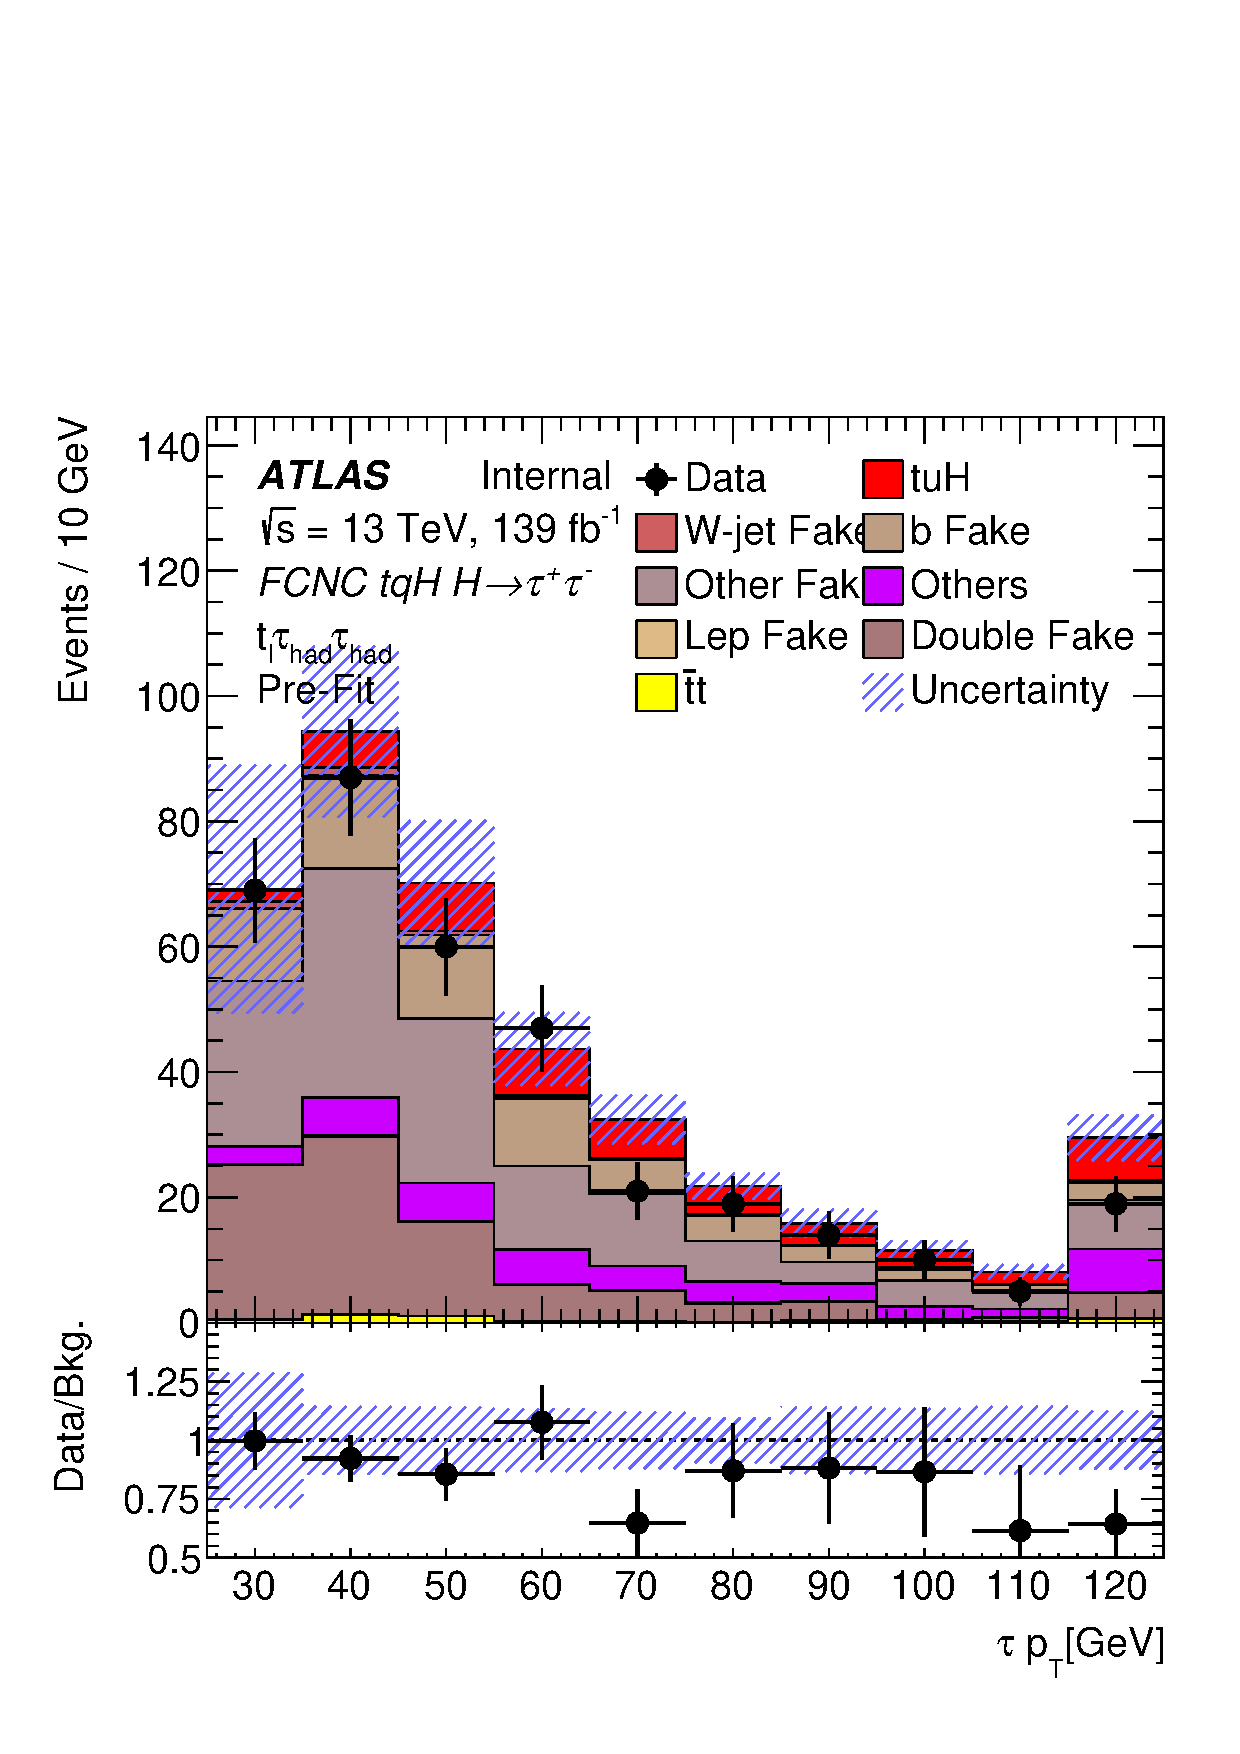
\includegraphics[page=1,width=0.33\textwidth]{figures/reg1l2tau1bnj_os.pdf} &
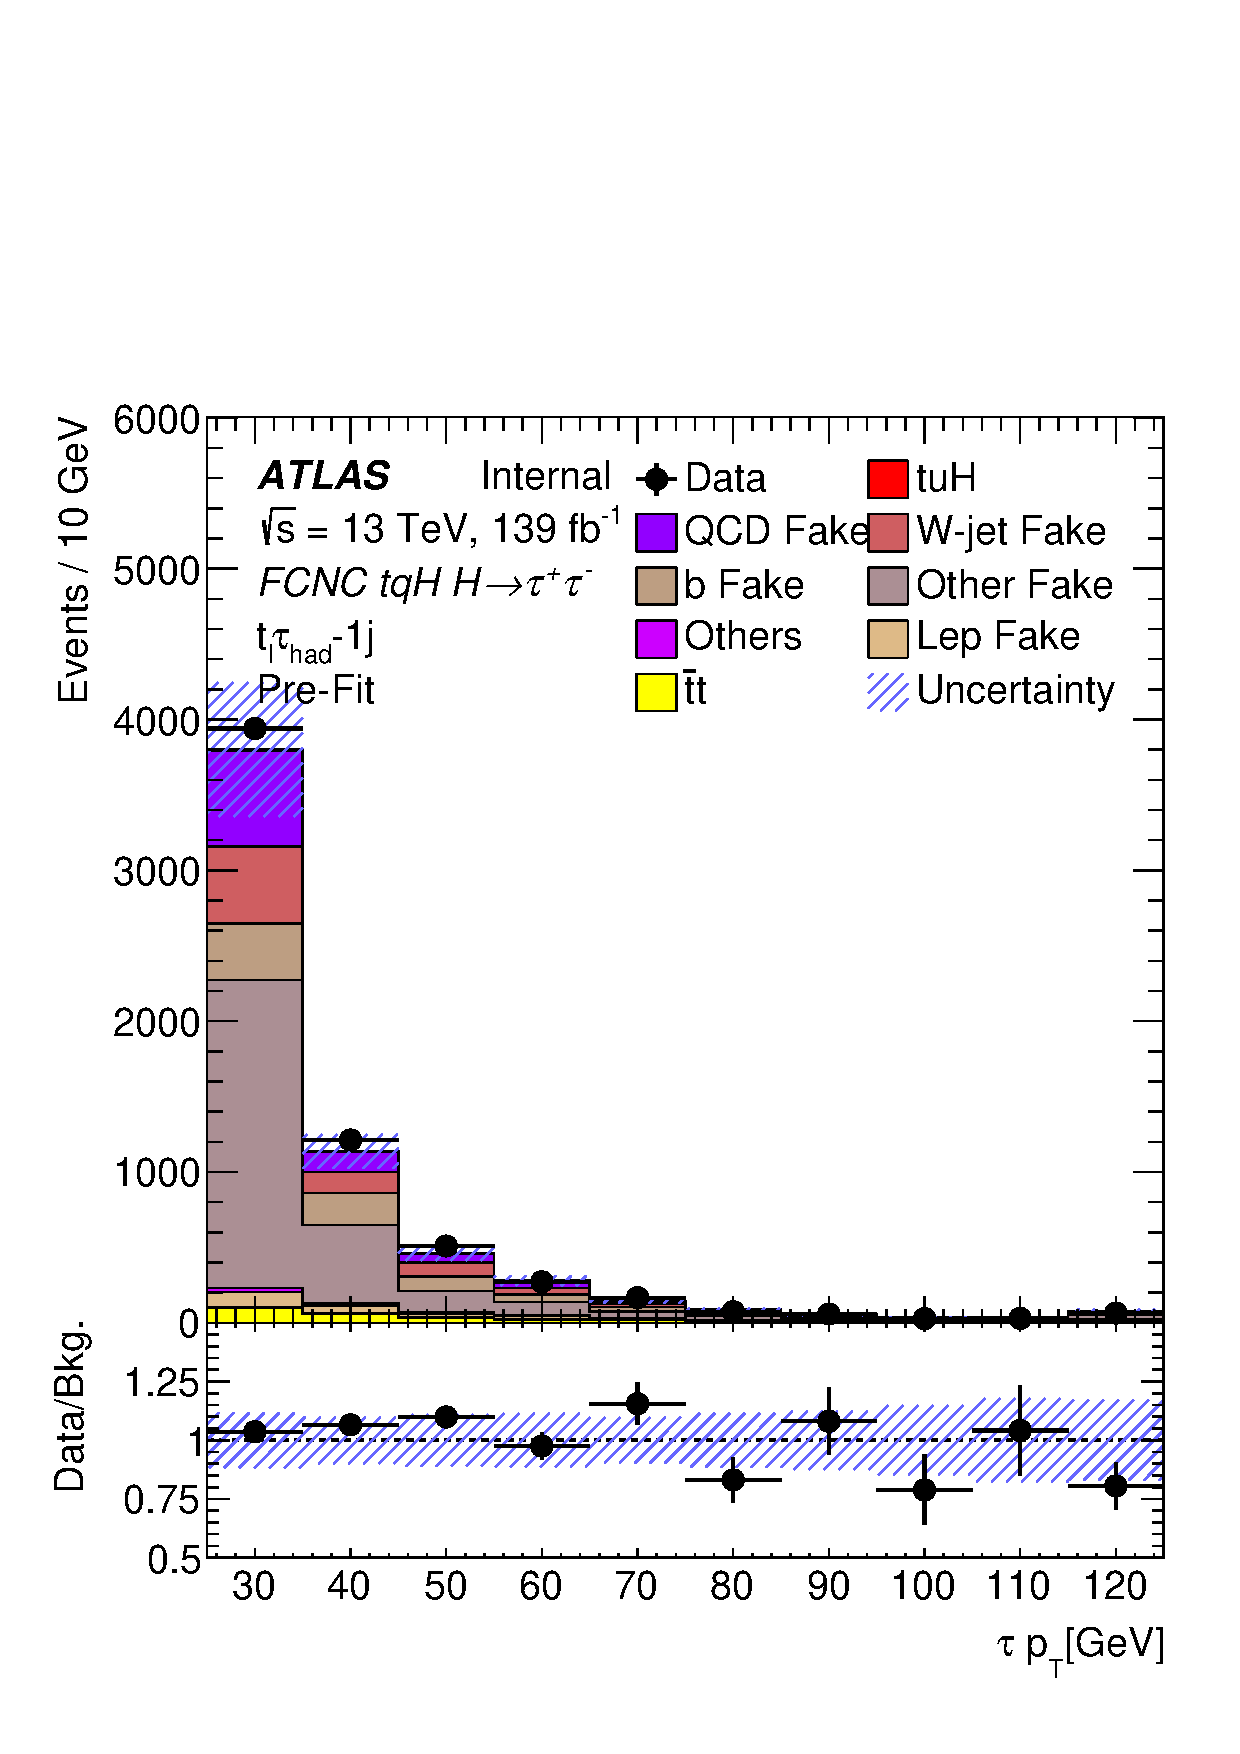
\includegraphics[page=1,width=0.33\textwidth]{figures/reg1l1tau1b1j_ss.pdf}&
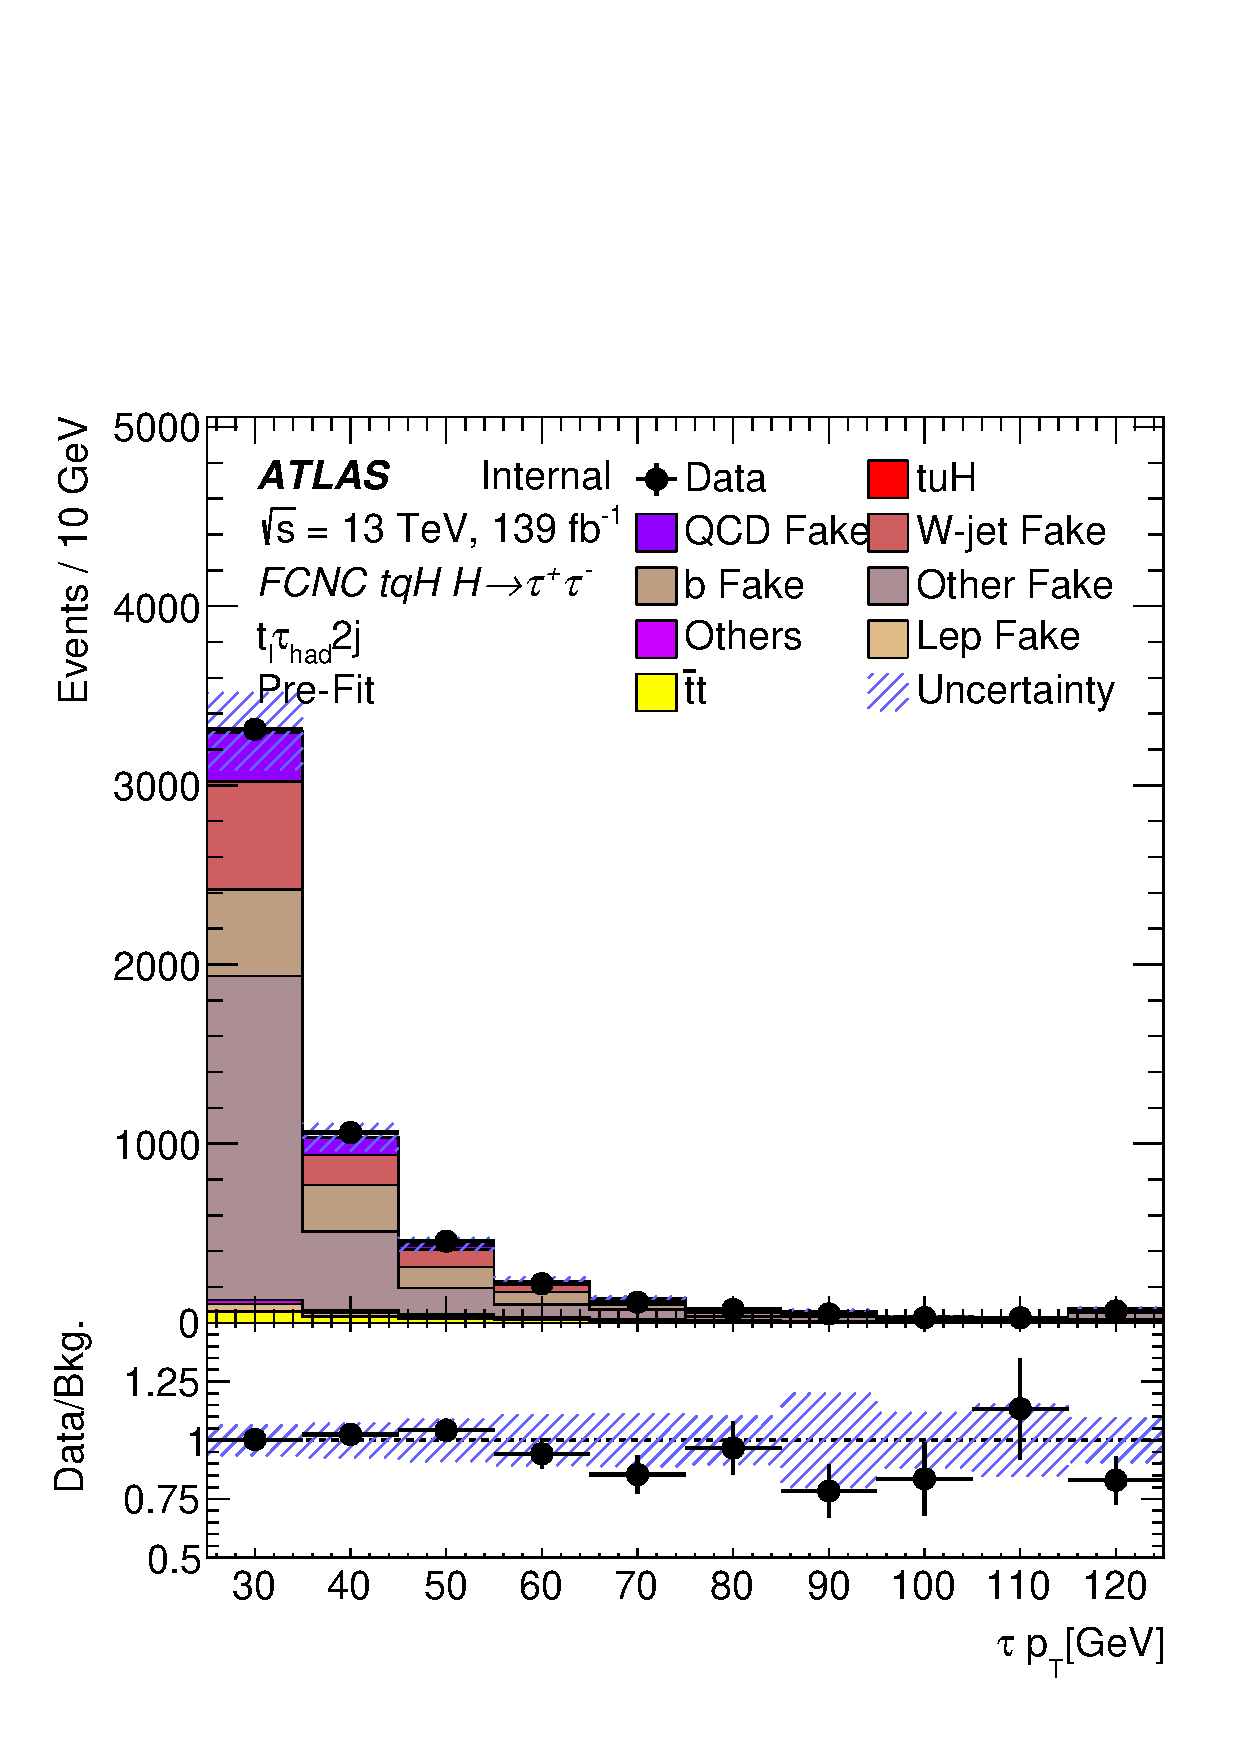
\includegraphics[page=1,width=0.33\textwidth]{figures/reg1l1tau1b2j_ss.pdf}\\
(a1) \pT(\tauhad) in $t_l\thadhad$ & (a2) \pT(\tauhad) in  $t_l\tauhad$-1j& (a3) \pT(\tauhad) in $t_l\tauhad$-2j\\
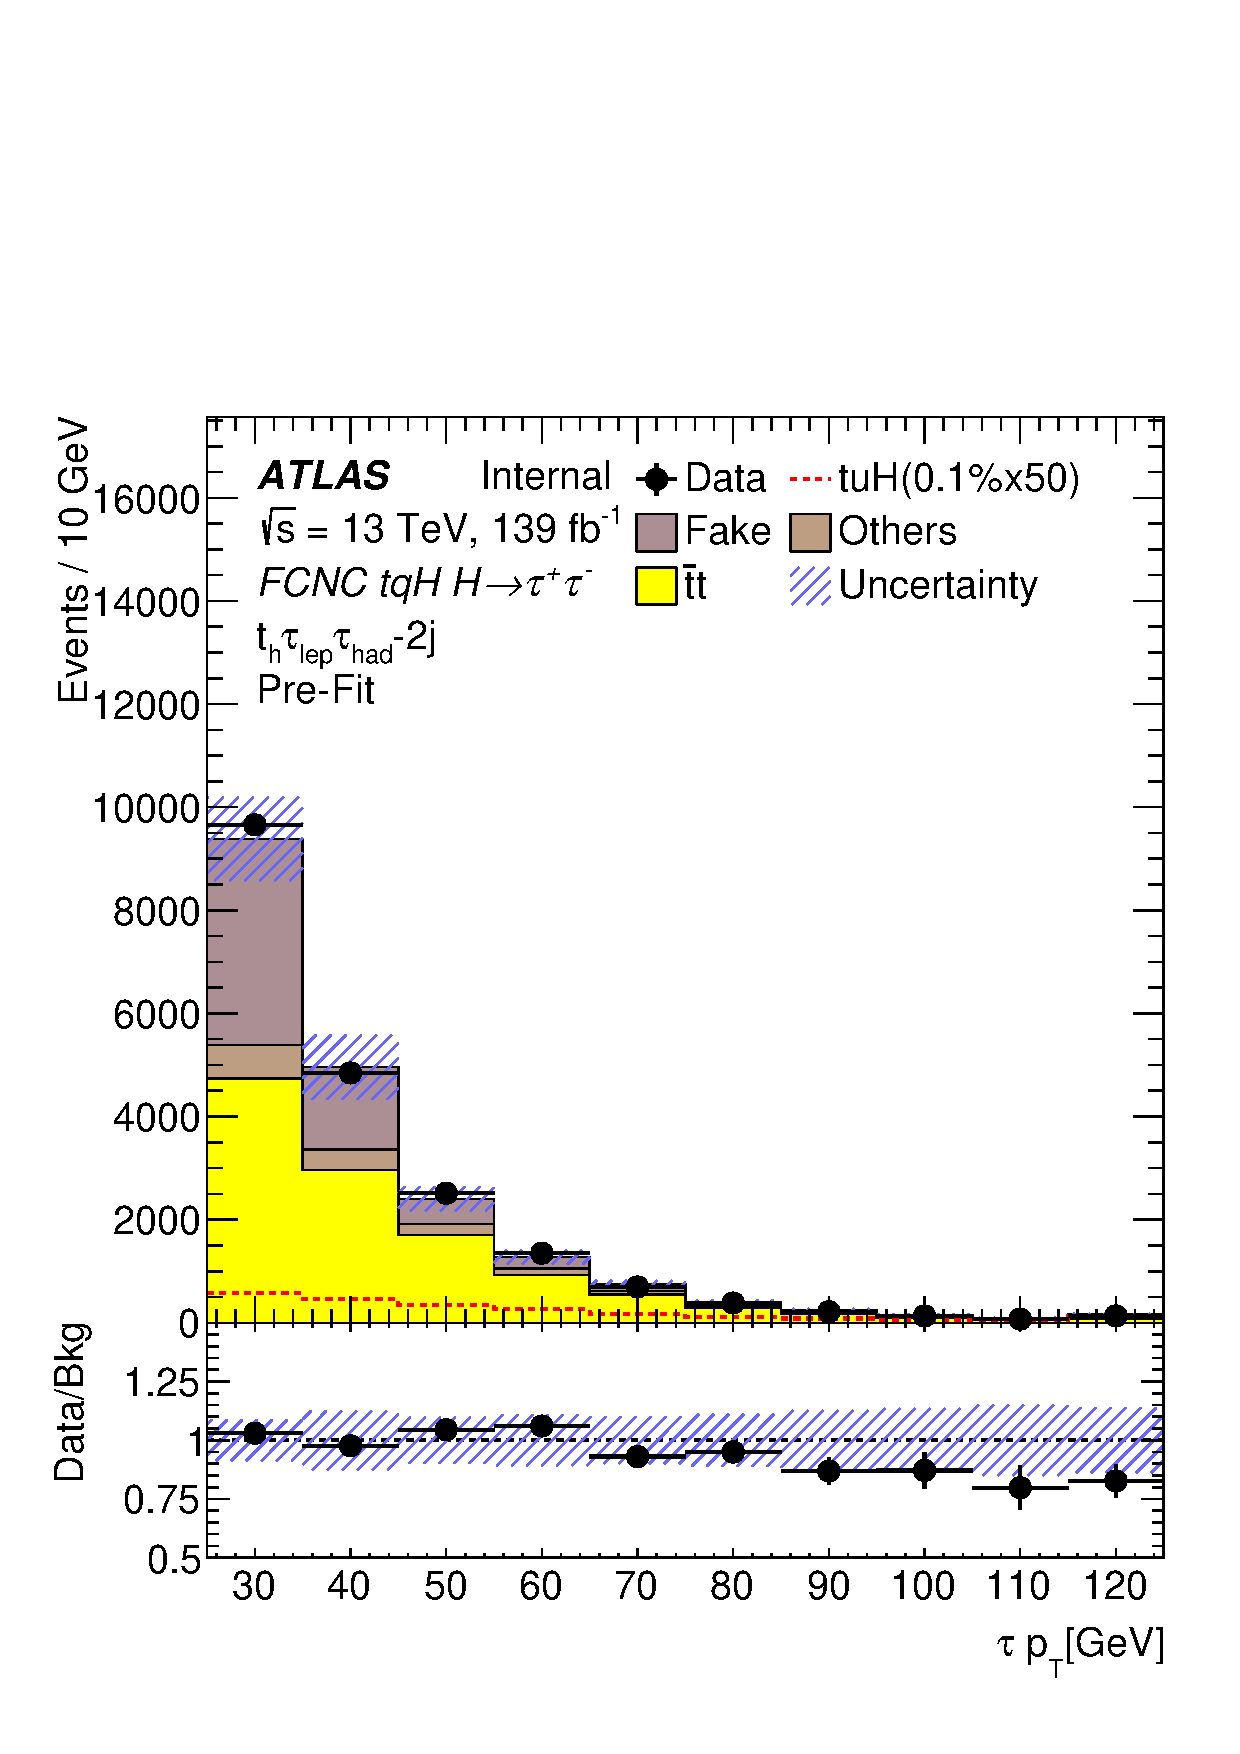
\includegraphics[page=1,width=0.33\textwidth]{figures/reg1l1tau1b2j_os.pdf}&
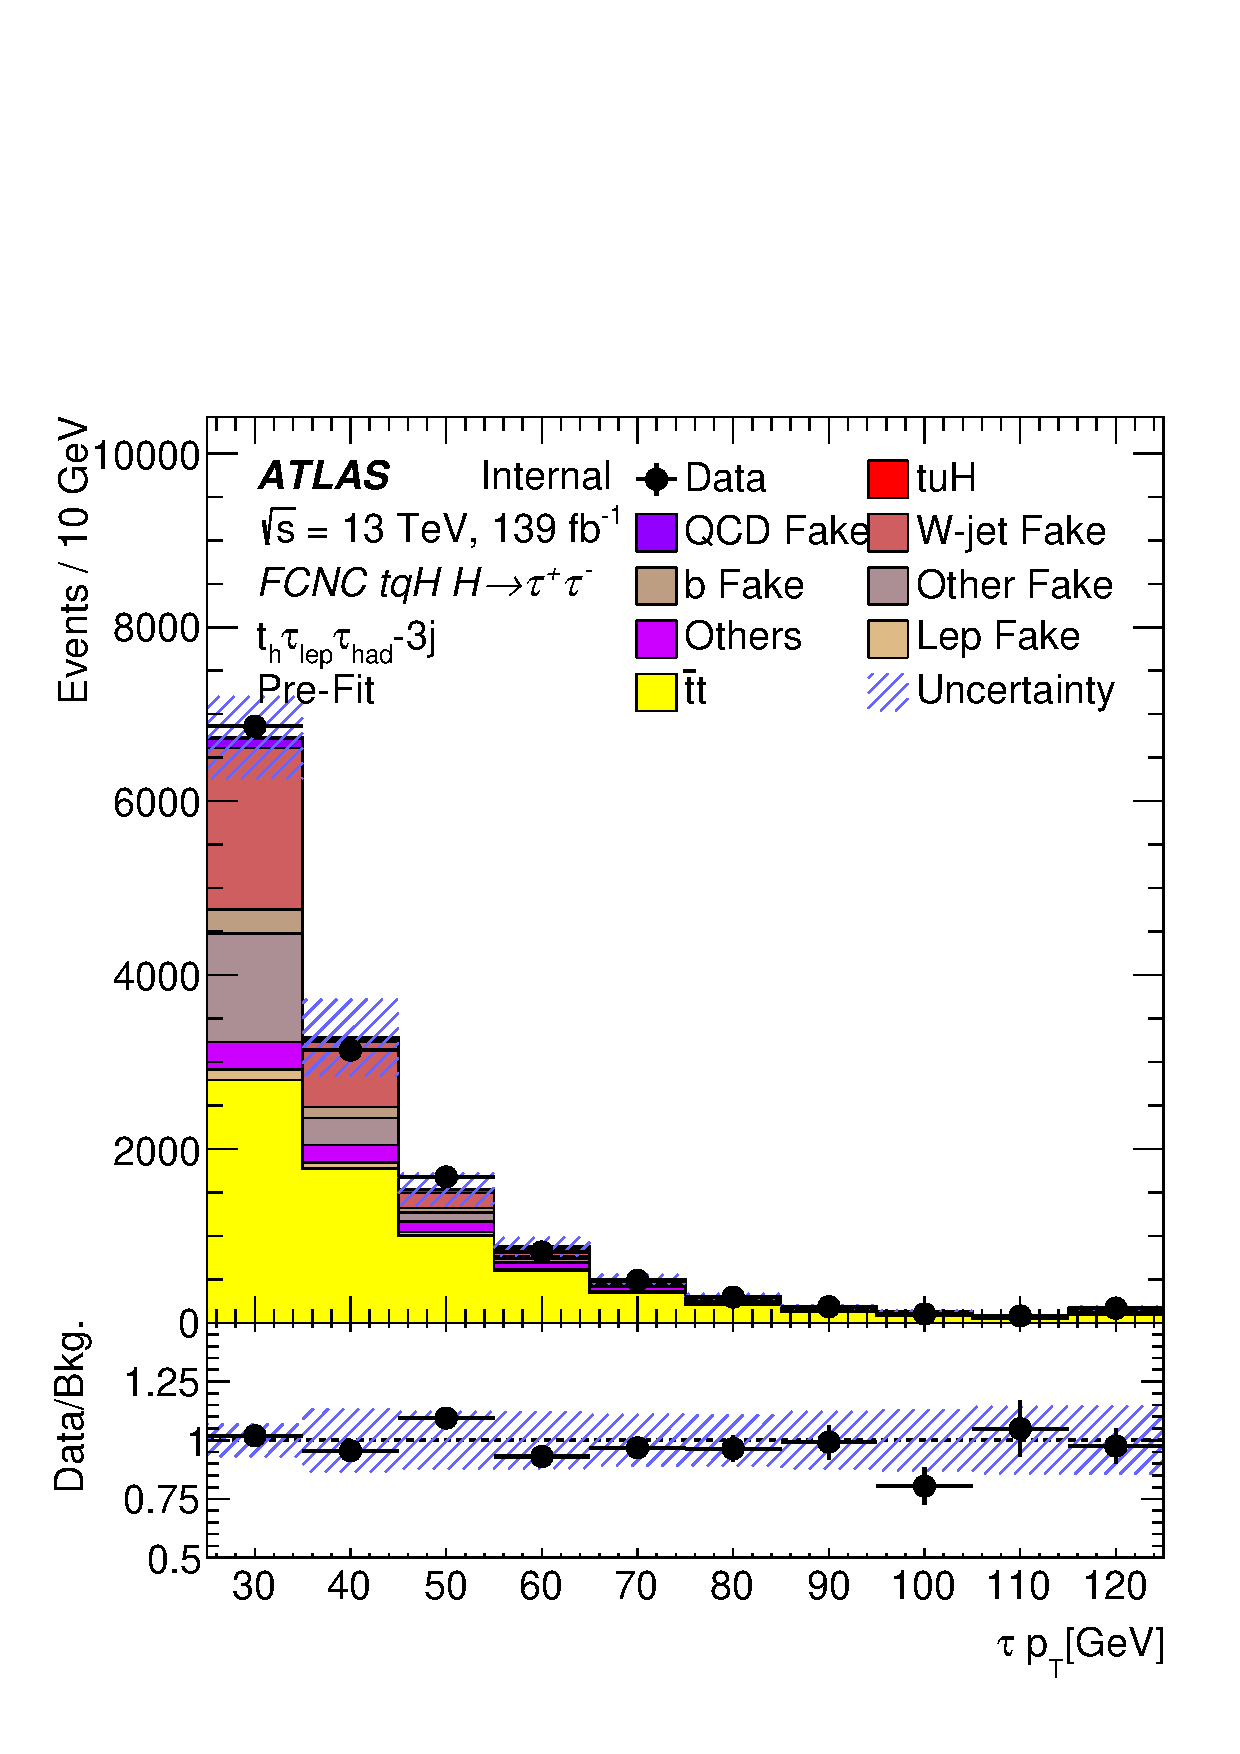
\includegraphics[page=1,width=0.33\textwidth]{figures/reg1l1tau1b3j_os.pdf}&
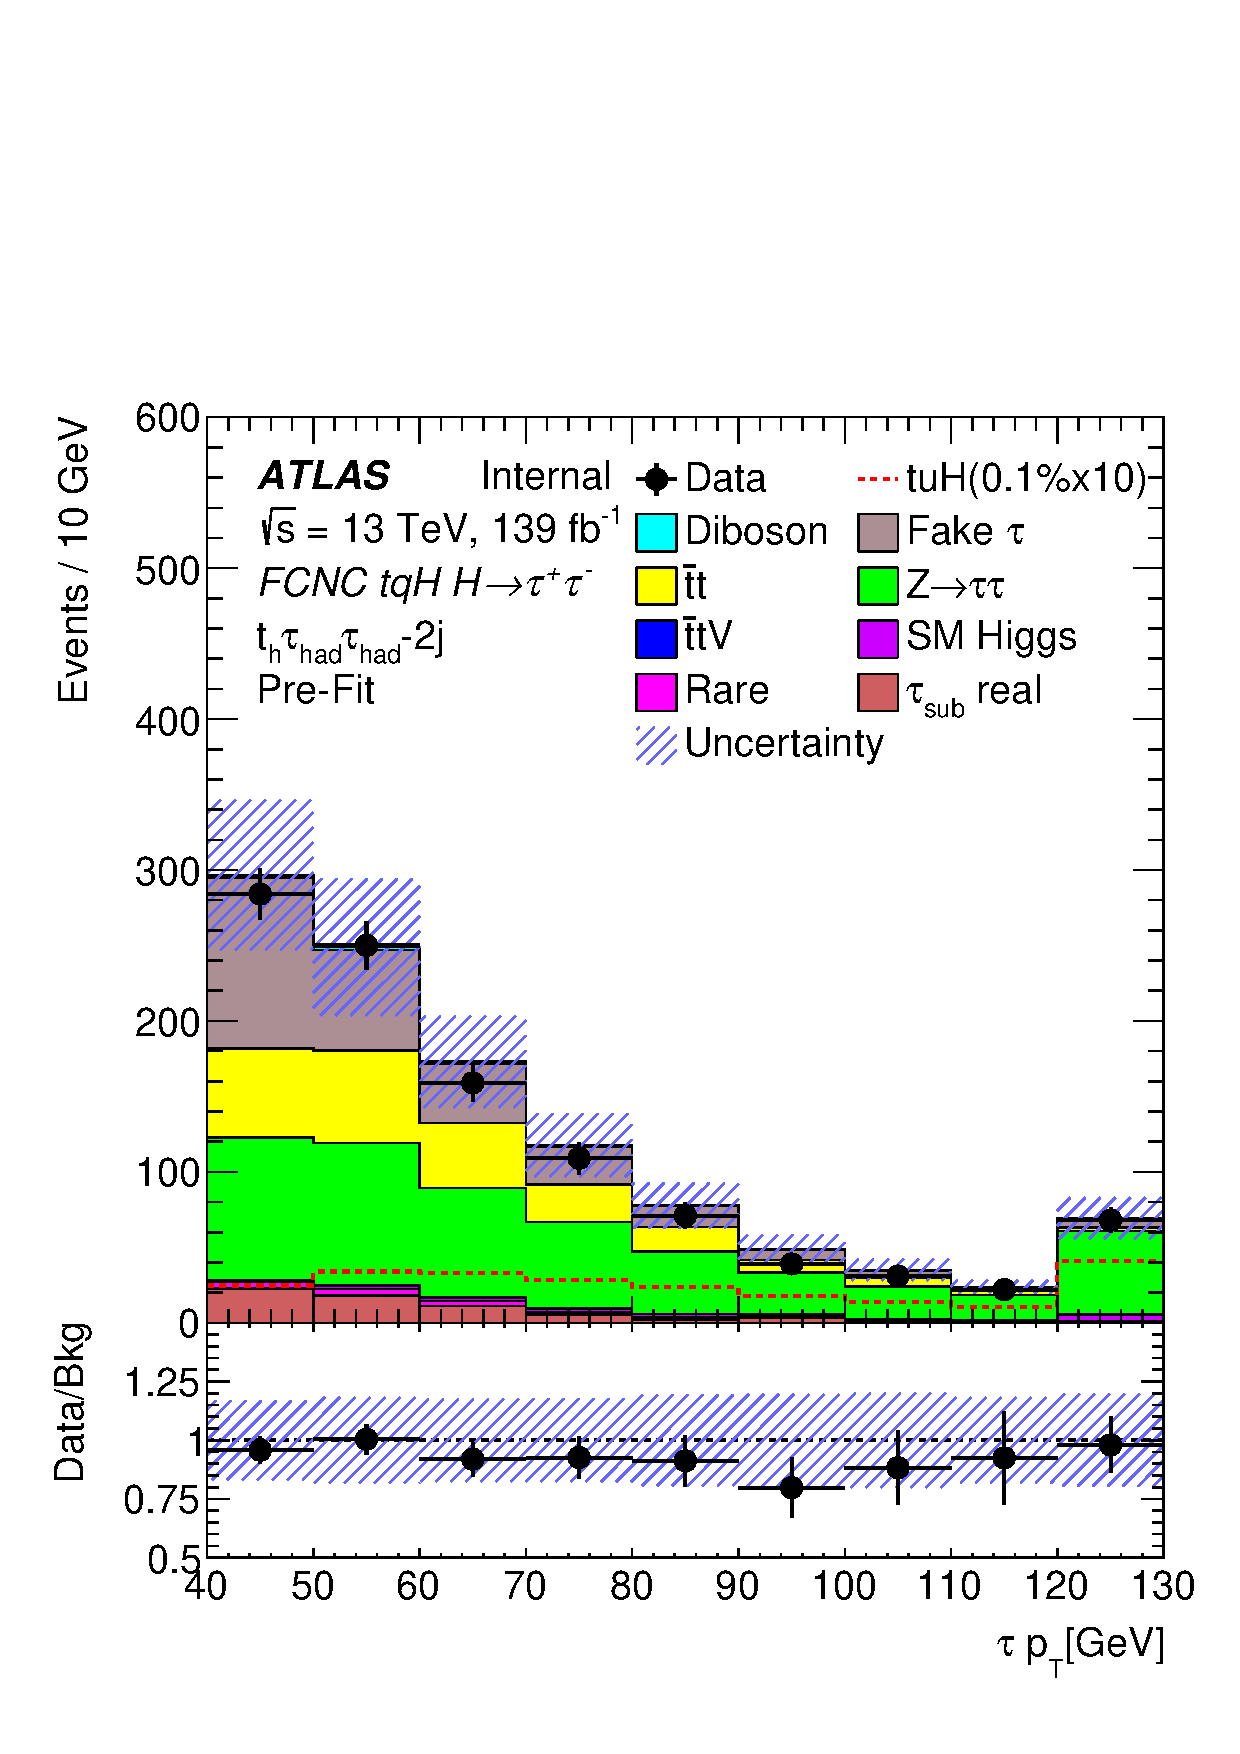
\includegraphics[page=1,width=0.33\textwidth]{figures/reg2mtau1b2jos_vetobtagwp70_highmet.pdf}\\
(b1) \pT(\tauhad) in $t_h\tlhad$-2j & (b2) \pT(\tauhad) in  $t_h\tlhad$-3j & (b3) \pT(\tauhad) in $t_h\thadhad$-2j \\
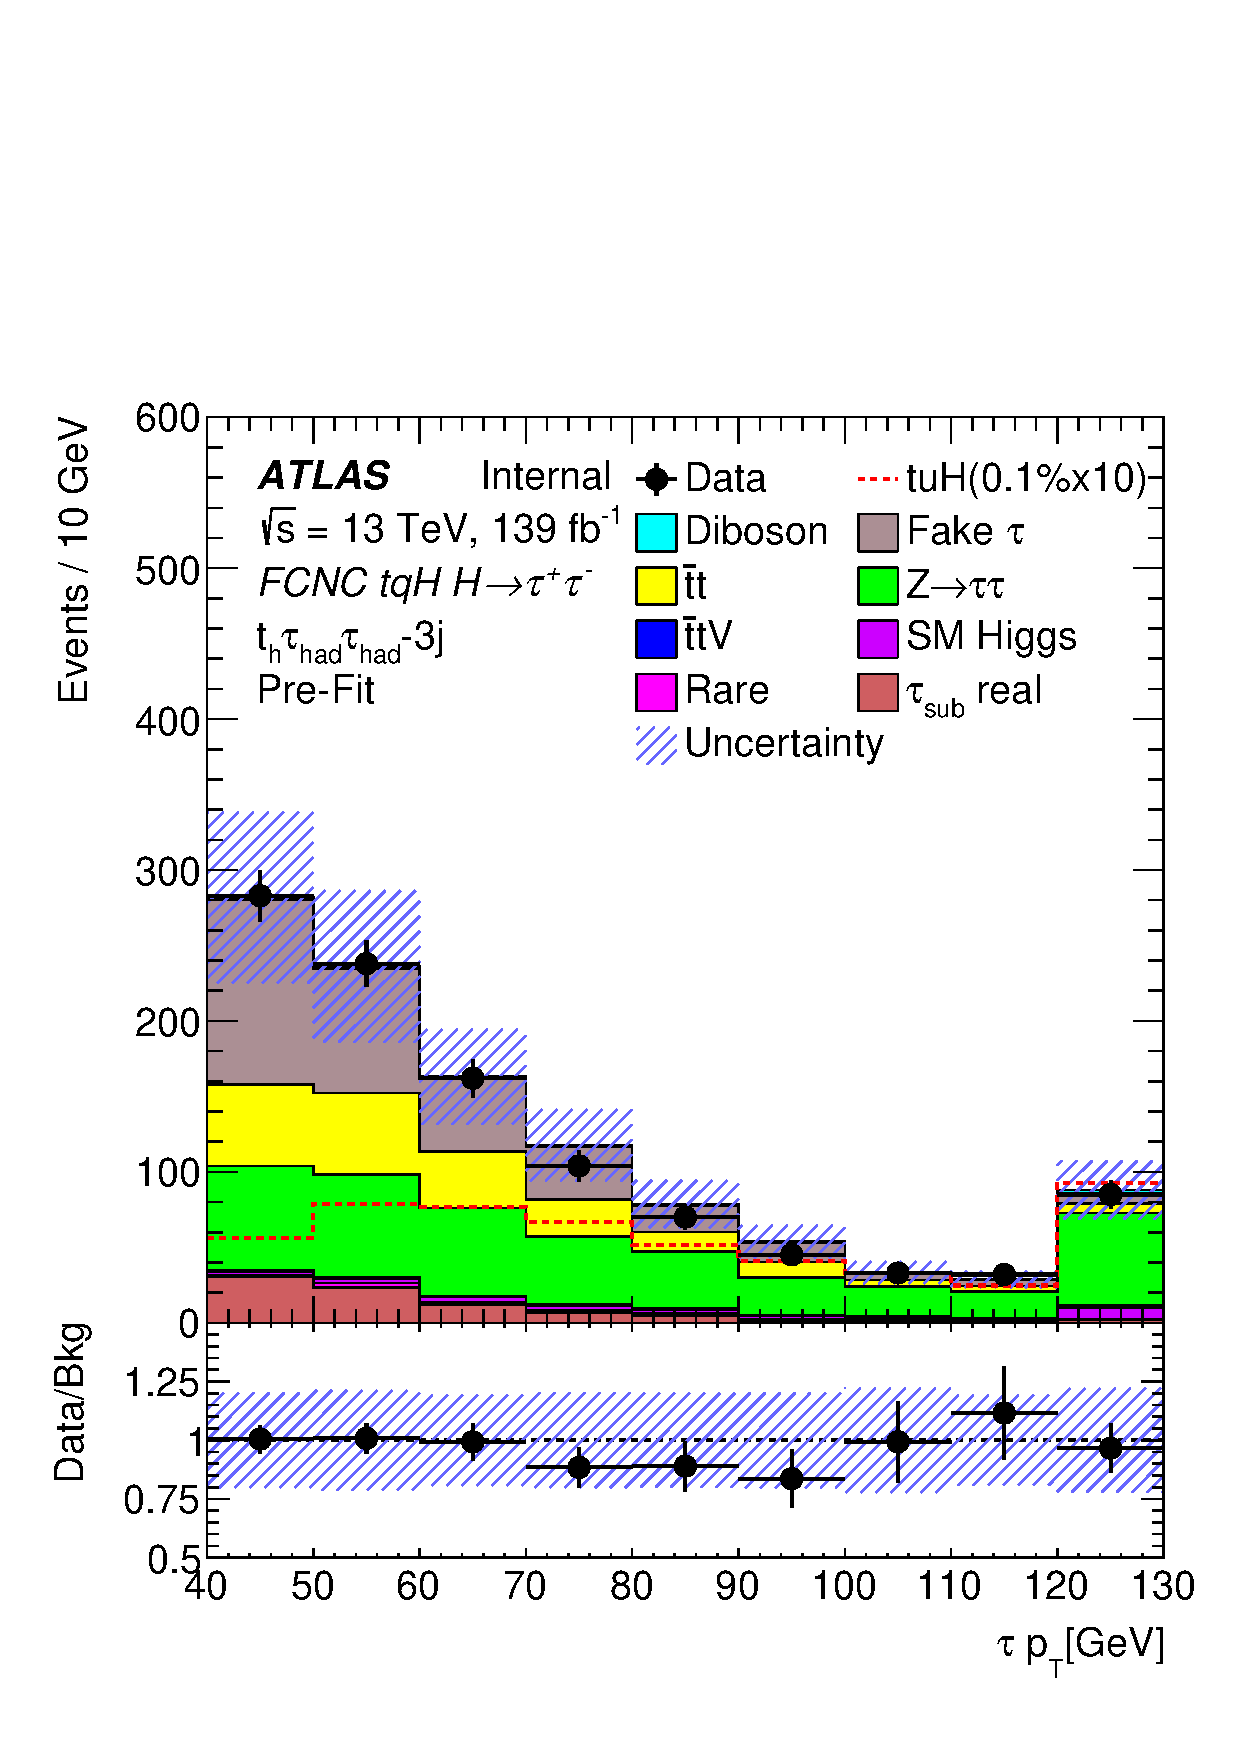
\includegraphics[page=1,width=0.33\textwidth]{figures/reg2mtau1b3jos_vetobtagwp70_highmet.pdf}&\\
(c1) \pT(\tauhad) in $t_h\thadhad$-3j\\
\end{tabular}
\caption{The leading $\thad$ $p_T$  distributions are compared between the expected background and $tuH$ signals in: $t_l\thadhad$ (a1),  $t_l\tauhad$-1j (a2),  $t_l\tauhad$-2j (a3), $t_h\tlhad$-2j (b1), $t_h\tlhad$-3j (b2), $t_h\thadhad$-2j (b3), and $t_h\thadhad$-3j (c1) before the fit to data ('Pre-Fit'). The uncertainty band includes both the statistical and systematic uncertainties in the background prediction. Underflow and overflow bins are included respectively in the first and last bins. Rare including single top, and V+jets and only subtau real refers to t$\bar{t}$ MC with leading tau faked by other object, subleading tau from real contribution. The lower panels show the ratios of the data ('Data') to the background prediction ('Bkg.')}
\label{fig:taupt_prefit}
\end{figure}




% %\input{\FCNCFigures/tex/BDT}
% \begin{figure}[H]
% \centering
% \begin{tabular}{@{}ccc@{}}
% \includegraphics[page=7,width=0.33\textwidth]{\FCNCFigures/tthML/showFake/faketau/postfit/NOMINAL_fancpaper/reg1l2tau1bnj_os/BDTG_test.pdf} &
% \includegraphics[page=7,width=0.33\textwidth]{\FCNCFigures/tthML/showFake/faketau/postfit/NOMINAL_fancpaper/reg1l1tau1b1j_ss_vetobtagwp70_highmet/BDTG_test.pdf}&
% \includegraphics[page=7,width=0.33\textwidth]{\FCNCFigures/tthML/showFake/faketau/postfit/NOMINAL_fancpaper/reg1l1tau1b2j_ss_vetobtagwp70_highmet/BDTG_test.pdf}\\
% (a1) BDT dicriminant in $t_l\thadhad$ & (a2) BDT dicriminant in  $t_l\tauhad$-1j& (a3) BDT dicriminant in $t_l\tauhad$-2j\\
% \includegraphics[page=7,width=0.33\textwidth]{\FCNCFigures/tthML/showFake/faketau/postfit/NOMINAL_fancpaper/reg1l1tau1b2j_os_vetobtagwp70_highmet/BDTG_test.pdf} &
% \includegraphics[page=7,width=0.33\textwidth]{\FCNCFigures/tthML/showFake/faketau/postfit/NOMINAL_fancpaper/reg1l1tau1b3j_os_vetobtagwp70_highmet/BDTG_test.pdf} &
% \includegraphics[page=7,width=0.33\textwidth]{\FCNCFigures/xTFW/showFake/NOMINAL/reg2mtau1b2jos_vetobtagwp70_highmet/BDTG_test.pdf} \\
% (b1) BDT dicriminant in $t_h\tlhad$-2j & (b2) BDT dicriminant in  $t_h\tlhad$-3j & (b3) BDT dicriminant in $t_h\thadhad$-2j \\
% \includegraphics[page=7,width=0.33\textwidth]{\FCNCFigures/xTFW/showFake/NOMINAL/reg2mtau1b3jos_vetobtagwp70_highmet/BDTG_test.pdf} & \\
% (c1) BDT dicriminant in$t_h\thadhad$-3j\\
% \end{tabular}
% \caption{ The BDT output distributions are compared between the expected background and $tqH$ signals in: $t_l\thadhad$ (a1),  $t_l\tauhad$-1j (a2),  $t_l\tauhad$-2j (a3),$t_h\tlhad$-2j (b1), $t_h\tlhad$-3j (b2), $t_h\thadhad$-2j (b3), and $t_h\thadhad$-3j (c1). Only statistical uncertainties are being shown (?). Underflow and overflow bins are included
% respectively in the first and last bins. Empty data bins here are always blinded based on our strategy. The real tau contributions shown from $t\bar{t}$ and other MC including % diboson, single top, and V+jets.}
% \label{fig:asimov_prefitbdt}
% \end{figure}

